\documentclass{article}

\usepackage[margin=0.5in,bottom=1in,footnotesep=1in]{geometry}

\usepackage{amsmath}

\usepackage{multicol}
\setlength{\columnsep}{1cm}
\usepackage[]{algorithm2e}

\usepackage{lipsum}% for dummy text
\usepackage[varg]{txfonts}
\usepackage{graphicx}
\usepackage{subcaption}
\usepackage{multirow}

\usepackage{titlesec}
\titleformat{\section}{\fontfamily{phv}\fontsize{12}{15}\bfseries}{\thesection}{1em}{}
\titleformat{\subsection}{\fontfamily{phv}\fontsize{10}{15}\itshape}{\thesubsection}{1em}{}

\title{\textbf{FYS4150 Project 1: \\1-dimensional Poisson equation}}
\author{Marie Foss, Maria Hammerstr{{\o}}m}
\date{} % removes date from title

\begin{document}

\maketitle

\begin{abstract}
	\noindent We explore the efficiency of two methods for solving a set of linear equations when the matrix involved is a tridiagonal matrix. The first method is a simplified algorithm that takes into account the simplicity of the tridiagonal matrix. The second method is an algorithm using a full LU decomposition, which will work for any matrix. We find that the simplified algorithm is superior when dealing with a large tridiagonal matrix, both with respect to accuracy of the result, as well as the computing time. 
	\vspace*{2ex}
\end{abstract}



\begin{multicols}{2}

\section{Introduction}
In this project we will solve the one-dimensional Poisson equation with Dirichlet boundary conditions. This is done by rewriting it as a set of linear equations, and solving these numerically in a program written in C++ \footnote{All files associated with the project are located at: https://github.com/mariahammerstrom/Project1}. The C++ program is accompanied by a MATLAB script which plots the results. 

The equation to be solved is
\begin{equation}\label{eq:Poisson}
	-u''(x) = f(x), \hspace{0.5cm} \mathrm{with } x\in(0,1) \mathrm{ and } u(0) = u(1) = 0.
\end{equation}
We define the discretized approximation to $u$ as $v_i$  with grid points $x_i=ih$ in the interval from $x_0=0$ to $x_{n+1}=1$. The step length or spacing is defined as $h=1/(n+1)$, and the boundary conditions are $v_0 = v_{n+1} = 0$. The second derivative of $u$ can be approximated to be
\begin{equation}\label{eq:second_derivative}
   -\frac{v_{i+1}+v_{i-1}-2v_i}{h^2} = f_i  \hspace{0.5cm} \mathrm{for} \hspace{0.1cm} i=1,\dots, n,
\end{equation}
where $f_i=f(x_i)$. Eq. (\ref{eq:second_derivative}) can be written as a linear set of equations of the form: 
\begin{equation}
	{\bf A}{\bf v} = \tilde{{\bf b}},
\end{equation}
where $\tilde{b}_i=h^2f_i$ and \textbf{A} is an $n\times n$ matrix of the form:
\begin{equation}
    {\bf A} = \left(\begin{array}{cccccc}
                           2& -1& 0 &\dots   & \dots &0 \\
                           -1 & 2 & -1 &0 &\dots &\dots \\
                           0&-1 &2 & -1 & 0 & \dots \\
                           & \dots   & \dots &\dots   &\dots & \dots \\
                           0&\dots   &  &-1 &2& -1 \\
                           0&\dots    &  & 0  &-1 & 2 \\
                      \end{array} \right)
\end{equation}
This can be shown by writing it out. We then get
\begin{align*}
	2v_1 - v_2 &= \tilde{b}_1 \\
	-v_1 + 2v_2 - v_3 &= \tilde{b}_2 \\
	-v_2 + 2v_3 - v_4 &= \tilde{b}_3 \\
	... \\
	-v_{i-1} + 2v_n - v_{i+1} &= \tilde{b}_i,
\end{align*}
which is the same as Eq. (\ref{eq:second_derivative}). 

We will assume that the source term is $f(x) = 100e^{-10x}$. Using the interval and boundary conditions as stated above, the above differential equation has a closed-form  solution given by $u(x) = 1-(1-e^{-10})x-e^{-10x}$. We will compare our numerical solution with this result. 





\section{Methods}
\subsection{Simple algorithm}
In our case we are dealing with a simple tridiagonal matrix. We can therefore rewrite our matrix \textbf{A} in terms of one-dimensional vectors \textit{a, b, c} of length 1:\textit{n}. The linear equation then reads
\begin{equation}
    {\bf A} = \left(\begin{array}{cccccc}
                           b_1& c_1 & 0 &\dots   & \dots &\dots \\
                           a_2 & b_2 & c_2 &\dots &\dots &\dots \\
                           & a_3 & b_3 & c_3 & \dots & \dots \\
                           & \dots   & \dots &\dots   &\dots & \dots \\
                           &   &  &a_{n-2}  &b_{n-1}& c_{n-1} \\
                           &    &  &   &a_n & b_n \\
                      \end{array} \right)\left(\begin{array}{c}
                           v_1\\
                           v_2\\
                           \dots \\
                          \dots  \\
                          \dots \\
                           v_n\\
                      \end{array} \right)
  =\left(\begin{array}{c}
                           \tilde{b}_1\\
                           \tilde{b}_2\\
                           \dots \\
                           \dots \\
                          \dots \\
                           \tilde{b}_n\\
                      \end{array} \right).
\end{equation}
This can be written as

\begin{equation}\label{eq:tridiagonal_system}
  a_iv_{i-1}+b_iv_i+c_iv_{i+1} = \tilde{b}_i
\end{equation}
for $i=1,2,\dots,n$. We want to find a simple algorithm to solve this set of equations. To do this, we can rewrite Eq. (\ref{eq:tridiagonal_system}) by a method of elimination, which will lead to a system where there is only one unknown. 

The first thing to do is to realize that Eq. (\ref{eq:tridiagonal_system}) gives a system of three equations,
\begin{align}
	b_1 v_1 + c_1 v_2 &= \tilde{b}_1, \hspace{0.5cm} i = 1  \\
	a_i v_{i-1} + b_i v_i + c_i v_{i+1} &= \tilde{b}_i, \hspace{0.5cm} i = 2, \dots, n - 1 \\
	a_n v_{n-1} + b_n v_n &= \tilde{b}_n, \hspace{0.5cm} i = n  ,
\end{align}
where the boundary conditions have been applied to simplify the equations. The idea now is to subtract one row with a scalar multiple of another to eliminate variables. First we want to eliminate $v_1$, this can be done by dividing the first equation by $b_i$, which gives:

\begin{equation}
	v_1 = \tilde{b}_1/b_1 - \frac{c_1}{b_1}v_2.
\end{equation}
Then we can follow the same approach to eliminate $v_i$ by dividing each equation by $b_i$,\\

\begin{equation}
	v_i = \tilde{b}_i/b_i - \frac{a_i}{b_i}v_{i-1} - \frac{c_i}{b_i}v_{i+1}
\end{equation}
Trying to insert $v_{i-1}$ into the equations for $v_i$ can prove to be difficult. After some algebra one finds that:

\begin{equation}\label{eq:fsi}
	v_i = \left( \tilde{b}_i - a_iv_{i-1} - c_iv_{i+1} \right)/\left( b_i - \frac{a_ic_{i-1}}{d_{i-1}} \right),
\end{equation}
where $d_{i-1} =  b_{i-1} - a_{i-1}c_{i-2}/d_{i-2}$, and $d_{2} = b_2 - a_2c_1/b_1$. This process is called forward substitution.

We then have an equation for each $v_n$, and can start going back. This is done with a backward substitution. As we see from Eq. (\ref{eq:fsi}), we have to add a term $-c_iv_{i+1}/d_i$. \\



\subsection{LU decomposition}
In addition to solving the linear second-order differential equation Eq. (\ref{eq:Poisson}) using the simple algorithm described above, we want to solve the equation using LU decomposition, then compare the results. Doing an LU decomposition, means rewriting matrix {\bf A} as a product of a lower triangular matrix {\bf L} and an upper triangular matrix {\bf U}, so that

\begin{equation*}
	{\bf A} = {\bf L}{\bf U}.
\end{equation*}
For the LU decomposition we will use the provided \verb@lib.cpp@ library.




\section{Results}    \label{sec:analysis}

\subsection{Comparing the analytical and numerical solution}
We can run our code for different values of $n$ and plot the analytical and numerical solution to see how well they correspond. For different values of $n$, see Fig.~\ref{fig:n-values}.

\begin{figure*}
\begin{center}
\begin{tabular}{cc}
  	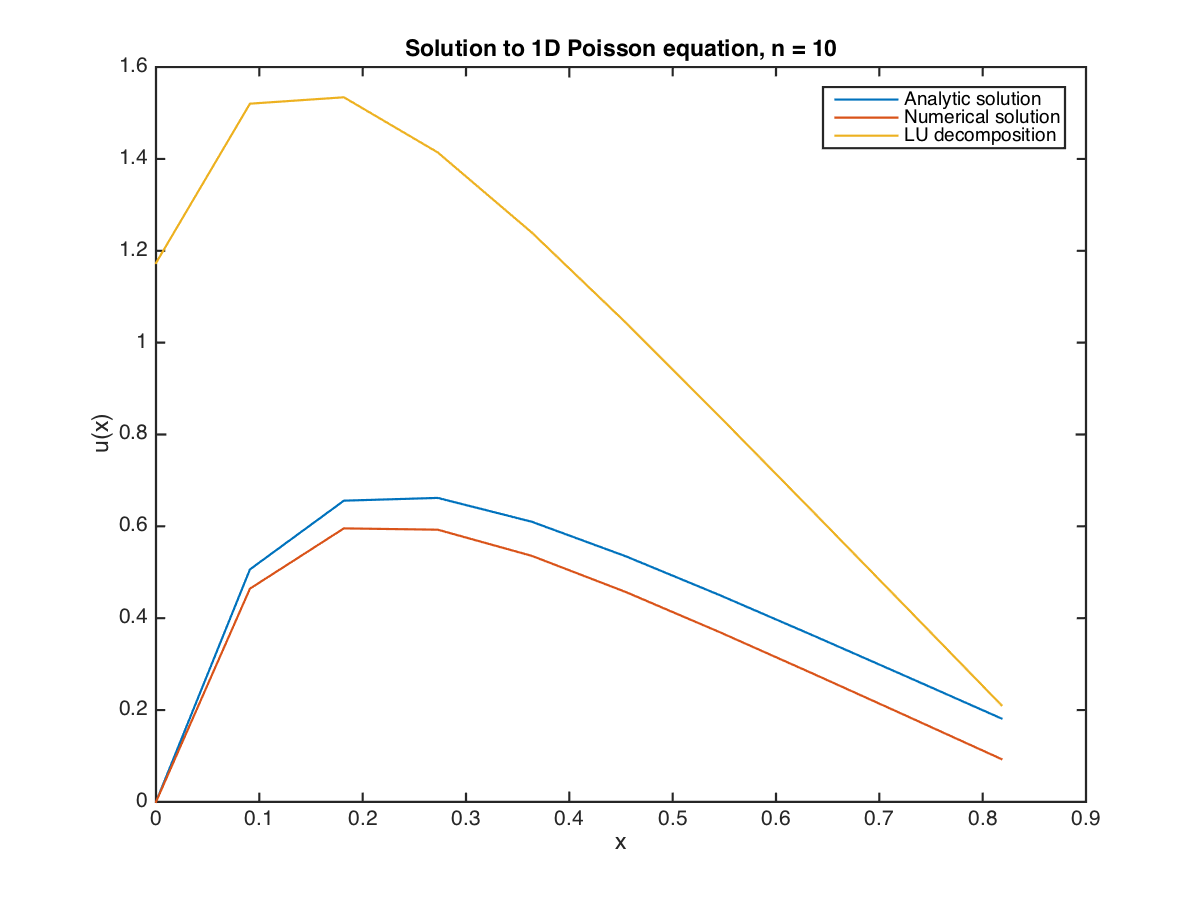
\includegraphics[width=90mm]{../build-Project1-Desktop_Qt_5_5_0_clang_64bit-Debug/Plot_n10.png} 	
	& 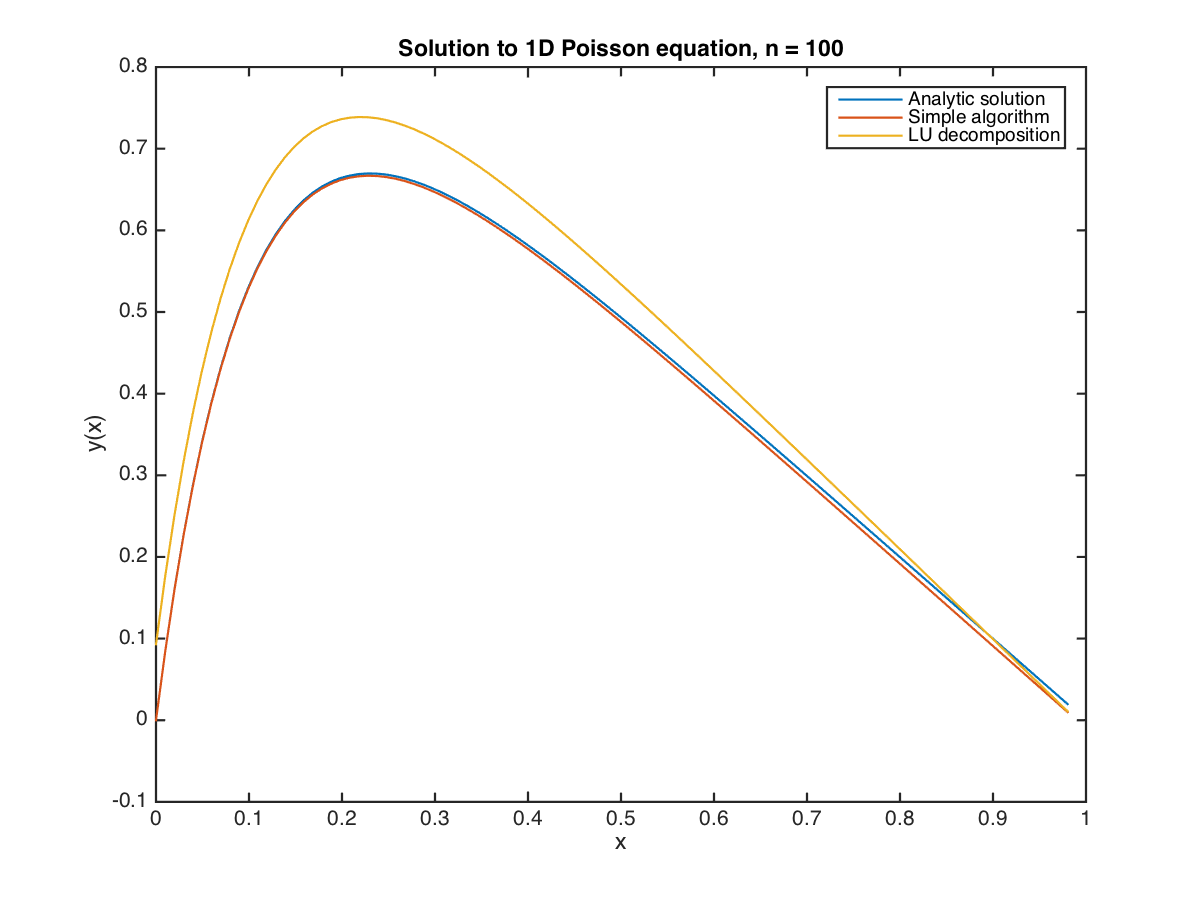
\includegraphics[width=90mm]{../build-Project1-Desktop_Qt_5_5_0_clang_64bit-Debug/Plot_n100.png} \\
	
	(a) $n$ = 10 								& (b) $n = 10^2$ \\[6pt]
	
 	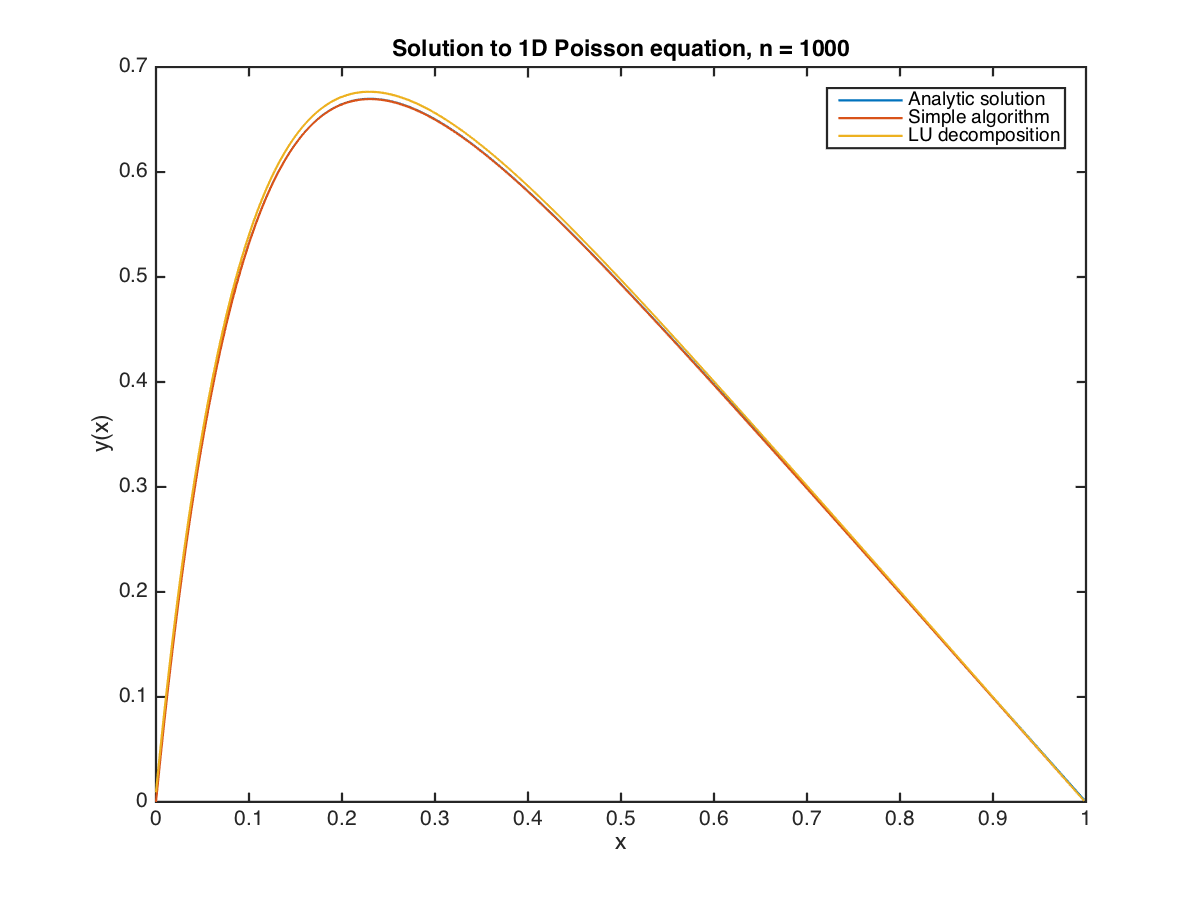
\includegraphics[width=90mm]{../build-Project1-Desktop_Qt_5_5_0_clang_64bit-Debug/Plot_n1000.png} 	
	& 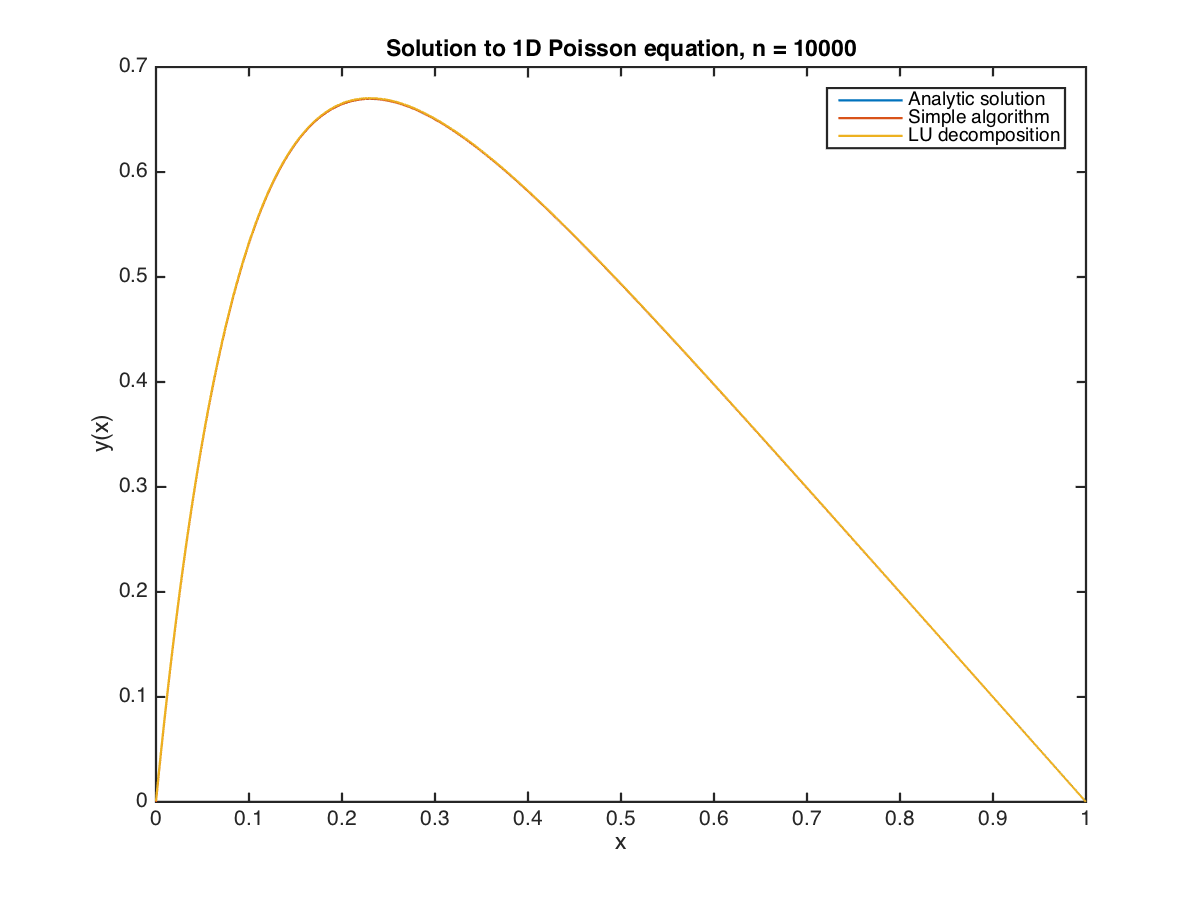
\includegraphics[width=90mm]{../build-Project1-Desktop_Qt_5_5_0_clang_64bit-Debug/Plot_n10000.png} \\
	(c) $n = 10^3$ 								& (d) $n = 10^4$ (still waiting on program) \\[6pt]
	
\end{tabular}
\caption{Comparison of the three different solutions for different values of $n$. In the three different cases $y(x) = u(x)$ (analytical solution, blue line), $y(x) = v(x)$ (simple algorithm, red line) and $y(x) = b(x)$ (LU decomposition, yellow line).}\label{fig:n-values}
\end{center}
\end{figure*}


\subsection{Relative errors}

The relative error in the data set is computed by calculating
\begin{equation}
   \epsilon_i=log_{10}\left(\left|\frac{v_i-u_i}
                 {u_i}\right|\right),
\end{equation}
for $i = 1, \dots, n$ for the function values $u_i$ and $v_i$, where $u_i$ represents the closed-form analytical solution, while $v_i$ is the numerical solution given by the simple algorithm described above. The relative error will be a function of $log_{10}(h)$. For each step length $h$ we want to extract the max value of the relative error. Doing this while increasing $n$ to $n=10000$ and $n=10^5$, gives the following results:

\begin{center}
\begin{tabular}{ l l }\hline
	$n$ 		&Maximum error (log$_{10}$) \\ \hline
	10 		& 1.18895 \\
	$10^2$  	& 1.03632 \\
	$10^3$ 	& 1.00786 \\
	$10^4$ 	& 1.00076 \\
	\hline
\end{tabular}
\end{center}

\begin{center}
Table 1: Maximum error as a function of step length.
\end{center}

\subsection{Number of floating point operations and time usage}
Some of the methods described above may be more computationally heavy for a computer to do than others. One way to evaluate this is to calculate the precise number of floating point operations ("FLOPS") needed to solve the equations.

Gaussian elimination requires $\frac{2}{3}n^3 + O(n^2)$ FLOPS and LU decomposition requires $O(n^3)$. By counting the floating point operations in our code, we find that for our tridiagonal system, $8n + 3$ FLOPS are required, where the number 3 represents the floating point operations outside of the \verb@for@-loops. 

The number of floating point operations and time usage in the different cases, are shown in the table below. A brute force Gaussian elimination is not used in the code in this project, and therefore has no values for time usage.


\begin{center}
    \begin{tabular}{ l  l  l  l } \hline
    \textbf{Method} 					&\textbf{\textit{n}} 	&\textbf{FLOPS} 	&\textbf{Time \textit{(s)}} \\ \hline
    \multirow{4}{*}{Simple algorithm} 		& 10 				& 8e+1			& 0 \\ 
    								& $10^2$  		& 8e+2 			& 0 \\
    								& $10^3$ 			& 8e+3 			& 0 \\ 
								& $10^4$ 			& 8e+4 			& 0 \\
    \hline
    \multirow{4}{*}{Gaussian elimination} 	& 10				& 1.6e+3			& - \\ 
    								& $10^2$  		& 1.51e+06		& - \\
    								& $10^3$ 			& 1.501e+09 		& - \\ 
								& $10^4$ 			& 1.5001e+12 		& - \\ 
    \hline
    \multirow{4}{*}{LU decomposition} 		& 10				& 1e+3			& 0 \\ 
    								& $10^2$ 			& 1e+06			& 0 \\
    								& $10^3$ 			& 1e+09			& 3 \\ 
								& $10^4$ 			& -7.2738e+08		& 6726 \\ 
    \hline
    \end{tabular}
\end{center}

\begin{center}
Table 2: The number of floating point operations and time usage by method.
\end{center}


\section{Conclusions} \label{sec:conclusions}
We ran our code with $n$ ranging from 10 to $10^4$. Due to the amount of time it took to compute the LU decomposition for $n = 10^4$, see Table 2, calculating $n = 10^5$ was impossible. 

In Fig.~\ref{fig:n-values} the results for the different $n$-values are shown. For $n = 10$ the result is way off for the LU decomposition, while the other two solutions are relatively close to each other. By only increasing $n$ by a factor of 10 the results improve significantly. The analytical solution and the solution of the simple algorithm are close to the same, while the result from the LU decomposition is lagging behind. Finally at $n = 10^3$ does all the three different methods align quite nicely, with the LU decomposition still slightly off, while at $n = 10^4$ does the results from all method coincide. 

If we look at this development with regards to computing time as well, shown in Table 2, we see that the computing time for the simple algorithm for our special case of a tridiagonal matrix, does not care about the increasing value of $n$, while the LU decomposition goes rapidly slower as $n$ is increased. Adding this to the fact that the result from the LU decomposition is not very impressive, the simple algorithm is a highly preferred method to use in this case.

If we review the results of the error analysis shown in Table 1, we see that the result is as expected: The error decreases as $n$ increases. For the largest value of $n$, the error is about zero (non-log scale).

From the calculations of the number of floating point operations in Table 2, we see that the simple algorithm continues to have a rather small number of FLOPS as $n$ increases, while Gaussian elimination and LU decomposition has quickly increasing number of FLOPS, which is the reason for the long time usage of the LU decomposition method. Something strange happens for the final FLOPS value for LU decomposition ...


\section{List of codes}

The codes developed for this project are:\\

\noindent \verb@main.cpp@ -- main program, C++

\noindent \verb@plotting.m@ -- plotting program, MATLAB
\end{multicols}

\end{document}
